% P9-T06: performance module by Le Thuong De (23120232).
% AI assistance: Codex helped draft and validate this module.
% Insert with % P9-T06: performance module by Le Thuong De (23120232).
% AI assistance: Codex helped draft and validate this module.
% Insert with % P9-T06: performance module by Le Thuong De (23120232).
% AI assistance: Codex helped draft and validate this module.
% Insert with % P9-T06: performance module by Le Thuong De (23120232).
% AI assistance: Codex helped draft and validate this module.
% Insert with \input{performance.tex} from the shared Beamer document.
\begin{frame}{How the experiment is controlled}
\begin{itemize}
\item One Tesla T4 session; one pinned source and binary for V0--V4.
\item Official dataset: 3 standard sites, 3 resolutions, plus challenge cases.
\item One warm-up and 5 measured runs per successful configuration.
\item Report stages, H2D, D2H, kernel total, and end-to-end separately.
\item Compare speedups only within the same measurement session.
\end{itemize}
\end{frame}

\begin{frame}{APOD: follow the measured bottleneck}
\begin{description}
\item[Assess] Identify the dominant stage using timing and Nsight.
\item[Parallelize] V1 moves the six-stage pipeline to CUDA.
\item[Optimize] V2/V3 target S5; V4 targets canvas construction in S6.
\item[Deploy] Preserve correctness, check memory safety, retain evidence.
\end{description}
\medskip
An improved stage can expose a different pipeline bottleneck.
\end{frame}

\begin{frame}{Why investigate S6 after V3?}
\centering
\begin{tabular}{lrr}
\toprule
P8, site2/large & V2 & V3 \\
\midrule
S5 (ms) & 30.538 & 12.200 \\
S6 (ms) & 29.580 & 28.468 \\
Pipeline total (ms) & 81.826 & 62.353 \\
\bottomrule
\end{tabular}
\medskip
\begin{itemize}
\item S6 accounts for 45.7\% of the V3 total in this historical run.
\item Even a 2$\times$ S6 speedup would allow only about 1.30$\times$ total speedup if everything else stayed constant.
\end{itemize}
\tiny Source: P8 report, 16 Nov 2026, same-session V2/V3; source checkout b3c79d7. Historical context only; P9 remeasures all versions.
\end{frame}

\begin{frame}{V4: single-pass canvas fusion}
\begin{block}{V3 renderer}
Clear canvas $\rightarrow$ copy A $\rightarrow$ gather and blend B.
\end{block}
\begin{block}{V4 renderer}
One thread per output pixel: test A/B validity, sample source pixels, blend, write RGB once.
\end{block}
\begin{itemize}
\item Keep canvas geometry, inverse projection, interpolation and rounding rules.
\item Reuse S1--S4 from V1 and S5 from V3.
\item Fewer passes suggest less traffic; hardware counters must verify actual DRAM traffic.
\end{itemize}
\end{frame}

\begin{frame}{Correctness before performance}
\begin{itemize}
\item P9-T02: six synthetic pairs and twelve real configurations on Tesla T4.
\item Accepted V4 source: \texttt{ab8df98d}; benchmark checks source equivalence.
\item Ten successful real cases: matching geometry and Max RGB = 0.
\item Challenge medium/large preserve the expected S6 NumericalFailure status.
\item Suite and production CLI memcheck: zero errors, zero bytes leaked.
\end{itemize}
\medskip
\tiny Source: docs/report/p9-v4-verification.md. Acceptance timing is excluded from benchmark tables.
\end{frame}

\begin{frame}{V4 benchmark: same-session comparison}
\input{generated/v4-table.tex}
\end{frame}

\begin{frame}{Nsight Systems shows three canvas operations become one}
\centering
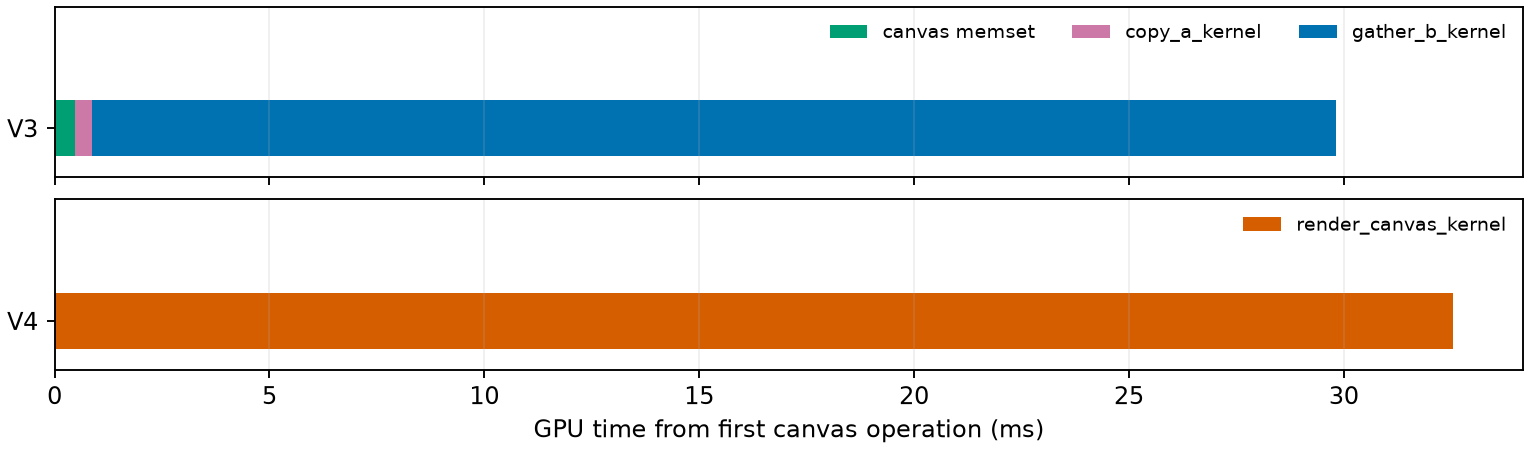
\includegraphics[width=.94\linewidth]{generated/nsys-v4.png}
\begin{itemize}
\item Tesla T4, site2/large, second pass of each trace.
\item V3 clear, copy A and gather B total 29.804 ms. V4 render takes 32.541 ms in this trace.
\item The five-run benchmark measures S6 at 28.712 ms for V3 and 28.190 ms for V4.
\end{itemize}
\end{frame}

\begin{frame}{Nsight Compute finds more DRAM traffic in sampled kernels}
\centering
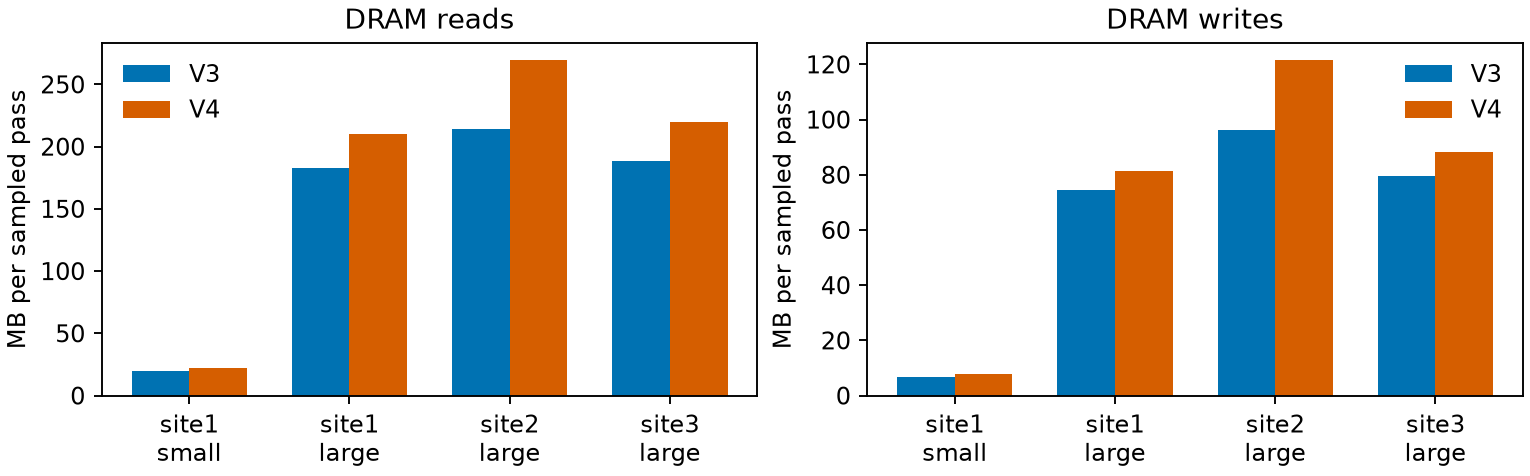
\includegraphics[width=.94\linewidth]{generated/ncu-v4.png}
\begin{itemize}
\item At site2/large, reads plus writes rise from 310.78 to 391.69 MB (+26.0\%).
\item The V3 bars sum one sample each of copy A and gather B. The V4 bars use one renderer sample. V3 canvas memset is outside the counter scope.
\end{itemize}
\end{frame}

\begin{frame}{What determines whether V4 is useful?}
\begin{itemize}
\item P9: V4 is faster in 8/9 standard cases; S6 geometric mean speedup is 1.0357$\times$.
\item Primary case paired blocks: median 1.0270$\times$, range 0.9774--1.0409$\times$; 4/5 blocks favor V4.
\item The primary case does not reach the previously proposed 5\% improvement threshold.
\item Keep challenge failures explicit; an absent timing is not zero time.
\item Separate profiler observations from unprofiled timing evidence.
\end{itemize}
\end{frame}

\begin{frame}{V5: dual-stream concurrency investigation}
\begin{block}{Two independent image branches}
Stream A and Stream B overlap H2D, S1, S2, and S3 concurrently; join before S4.
\end{block}
\begin{itemize}
\item Pre-S4 duration at site2/large decreases from $\sim$15.29 ms to $\sim$12.68 ms (1.207$\times$).
\item End-to-end speedup is modest (1.027$\times$ geometric mean) because downstream S5 and S6 dominate total time and SM resources are shared.
\item Confirms correctness and memory safety (0 memcheck errors, bit-for-bit parity with sequential mode).
\item Conclusion: V4 remains the production version; V5 serves as a concurrent stream case study.
\end{itemize}
\end{frame}

\begin{frame}{Lessons and limits}
\begin{itemize}
\item Faster S5 exposes S6; stage speedup is bounded by its pipeline share.
\item Fusion removes canvas passes. The sampled kernels show higher DRAM traffic.
\item Occupancy and throughput explain behavior; they are not the performance objective.
\item Preserve hashes, commands, raw runs, failures and original reports.
\item P9: total speedup is only 1.0086$\times$ (geometric mean); the benefit is modest.
\end{itemize}
\end{frame}
 from the shared Beamer document.
\begin{frame}{How the experiment is controlled}
\begin{itemize}
\item One Tesla T4 session; one pinned source and binary for V0--V4.
\item Official dataset: 3 standard sites, 3 resolutions, plus challenge cases.
\item One warm-up and 5 measured runs per successful configuration.
\item Report stages, H2D, D2H, kernel total, and end-to-end separately.
\item Compare speedups only within the same measurement session.
\end{itemize}
\end{frame}

\begin{frame}{APOD: follow the measured bottleneck}
\begin{description}
\item[Assess] Identify the dominant stage using timing and Nsight.
\item[Parallelize] V1 moves the six-stage pipeline to CUDA.
\item[Optimize] V2/V3 target S5; V4 targets canvas construction in S6.
\item[Deploy] Preserve correctness, check memory safety, retain evidence.
\end{description}
\medskip
An improved stage can expose a different pipeline bottleneck.
\end{frame}

\begin{frame}{Why investigate S6 after V3?}
\centering
\begin{tabular}{lrr}
\toprule
P8, site2/large & V2 & V3 \\
\midrule
S5 (ms) & 30.538 & 12.200 \\
S6 (ms) & 29.580 & 28.468 \\
Pipeline total (ms) & 81.826 & 62.353 \\
\bottomrule
\end{tabular}
\medskip
\begin{itemize}
\item S6 accounts for 45.7\% of the V3 total in this historical run.
\item Even a 2$\times$ S6 speedup would allow only about 1.30$\times$ total speedup if everything else stayed constant.
\end{itemize}
\tiny Source: P8 report, 16 Nov 2026, same-session V2/V3; source checkout b3c79d7. Historical context only; P9 remeasures all versions.
\end{frame}

\begin{frame}{V4: single-pass canvas fusion}
\begin{block}{V3 renderer}
Clear canvas $\rightarrow$ copy A $\rightarrow$ gather and blend B.
\end{block}
\begin{block}{V4 renderer}
One thread per output pixel: test A/B validity, sample source pixels, blend, write RGB once.
\end{block}
\begin{itemize}
\item Keep canvas geometry, inverse projection, interpolation and rounding rules.
\item Reuse S1--S4 from V1 and S5 from V3.
\item Fewer passes suggest less traffic; hardware counters must verify actual DRAM traffic.
\end{itemize}
\end{frame}

\begin{frame}{Correctness before performance}
\begin{itemize}
\item P9-T02: six synthetic pairs and twelve real configurations on Tesla T4.
\item Accepted V4 source: \texttt{ab8df98d}; benchmark checks source equivalence.
\item Ten successful real cases: matching geometry and Max RGB = 0.
\item Challenge medium/large preserve the expected S6 NumericalFailure status.
\item Suite and production CLI memcheck: zero errors, zero bytes leaked.
\end{itemize}
\medskip
\tiny Source: docs/report/p9-v4-verification.md. Acceptance timing is excluded from benchmark tables.
\end{frame}

\begin{frame}{V4 benchmark: same-session comparison}
% Generated from same-session P9 CSV; source ba97ed7, 2026-11-19.
\scriptsize
\centering
\begin{tabular}{llrrrr}
\toprule
Site & Size & V3 ms & V4 ms & Total speedup & S6 speedup \\
\midrule
site1 & small & 32.620 & 32.716 & 0.9971$\times$ & 1.0359$\times$ \\
site1 & medium & 31.027 & 30.785 & 1.0078$\times$ & 1.0633$\times$ \\
site1 & large & 108.107 & 107.157 & 1.0089$\times$ & 1.0061$\times$ \\
site2 & small & 21.415 & 21.142 & 1.0129$\times$ & 1.0368$\times$ \\
site2 & medium & 27.932 & 27.581 & 1.0127$\times$ & 1.0495$\times$ \\
site2 & large & 62.874 & 62.197 & 1.0109$\times$ & 1.0185$\times$ \\
site3 & small & 44.846 & 44.576 & 1.0061$\times$ & 1.0193$\times$ \\
site3 & medium & 56.167 & 55.723 & 1.0080$\times$ & 1.0403$\times$ \\
site3 & large & 101.713 & 100.393 & 1.0131$\times$ & 1.0525$\times$ \\
\bottomrule
\end{tabular}
\par\medskip Geometric mean total: 1.0086$\times$; S6: 1.0357$\times$.
\par One T4 session, one warm-up + 5 runs; nine standard cases.
\par\tiny Source: P9-T05, 19 Nov 2026, ba97ed7. Challenge failures excluded.

\end{frame}

\begin{frame}{Nsight Systems shows three canvas operations become one}
\centering
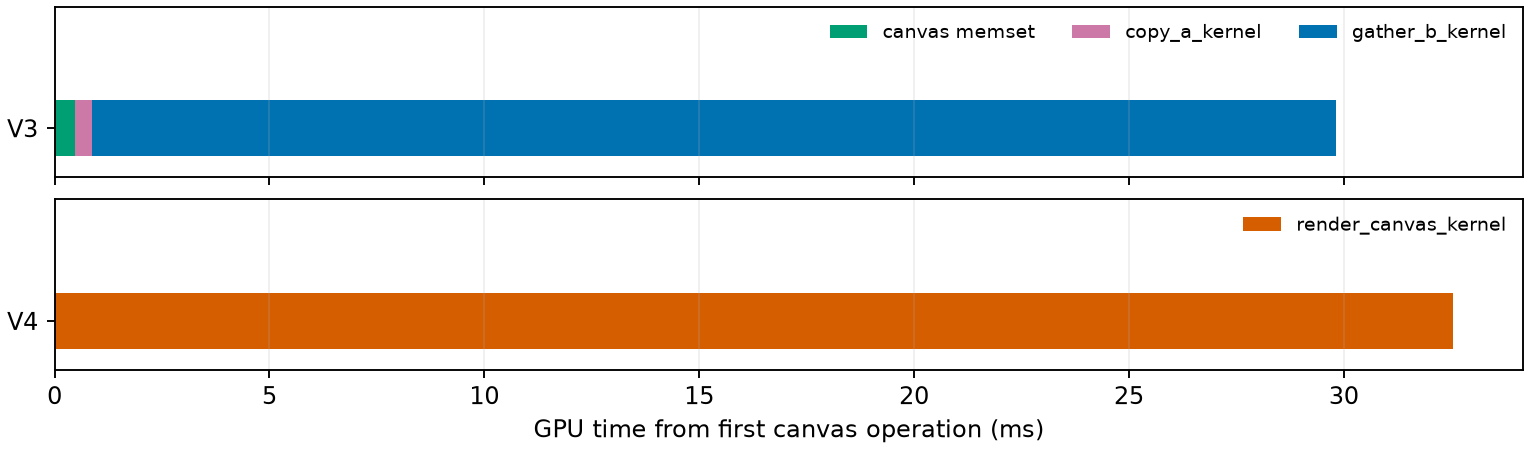
\includegraphics[width=.94\linewidth]{generated/nsys-v4.png}
\begin{itemize}
\item Tesla T4, site2/large, second pass of each trace.
\item V3 clear, copy A and gather B total 29.804 ms. V4 render takes 32.541 ms in this trace.
\item The five-run benchmark measures S6 at 28.712 ms for V3 and 28.190 ms for V4.
\end{itemize}
\end{frame}

\begin{frame}{Nsight Compute finds more DRAM traffic in sampled kernels}
\centering
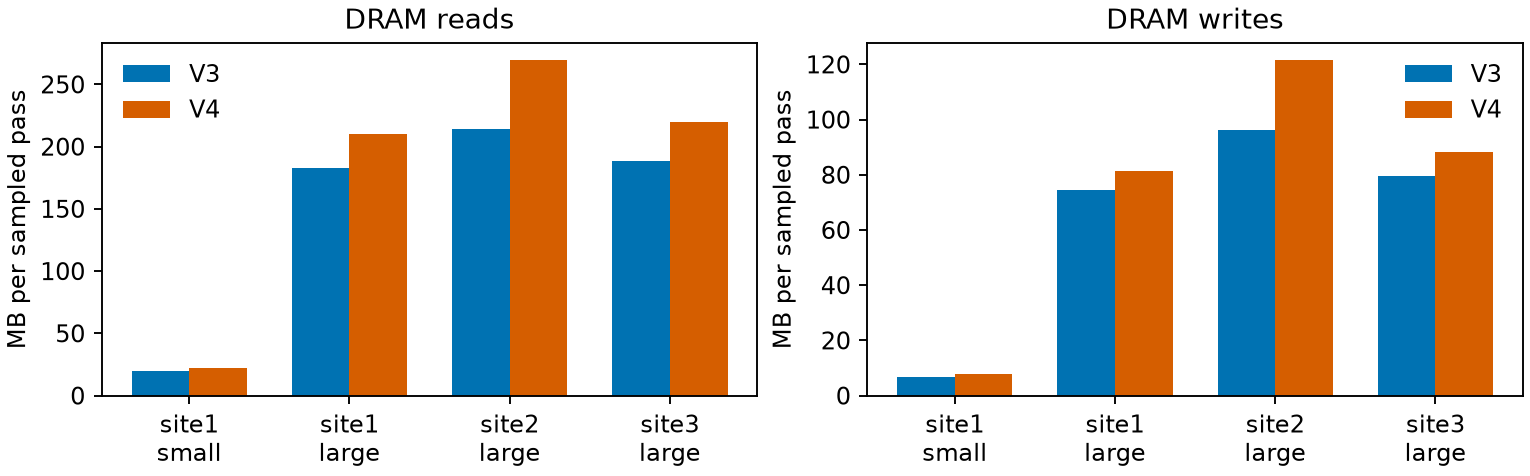
\includegraphics[width=.94\linewidth]{generated/ncu-v4.png}
\begin{itemize}
\item At site2/large, reads plus writes rise from 310.78 to 391.69 MB (+26.0\%).
\item The V3 bars sum one sample each of copy A and gather B. The V4 bars use one renderer sample. V3 canvas memset is outside the counter scope.
\end{itemize}
\end{frame}

\begin{frame}{What determines whether V4 is useful?}
\begin{itemize}
\item P9: V4 is faster in 8/9 standard cases; S6 geometric mean speedup is 1.0357$\times$.
\item Primary case paired blocks: median 1.0270$\times$, range 0.9774--1.0409$\times$; 4/5 blocks favor V4.
\item The primary case does not reach the previously proposed 5\% improvement threshold.
\item Keep challenge failures explicit; an absent timing is not zero time.
\item Separate profiler observations from unprofiled timing evidence.
\end{itemize}
\end{frame}

\begin{frame}{V5: dual-stream concurrency investigation}
\begin{block}{Two independent image branches}
Stream A and Stream B overlap H2D, S1, S2, and S3 concurrently; join before S4.
\end{block}
\begin{itemize}
\item Pre-S4 duration at site2/large decreases from $\sim$15.29 ms to $\sim$12.68 ms (1.207$\times$).
\item End-to-end speedup is modest (1.027$\times$ geometric mean) because downstream S5 and S6 dominate total time and SM resources are shared.
\item Confirms correctness and memory safety (0 memcheck errors, bit-for-bit parity with sequential mode).
\item Conclusion: V4 remains the production version; V5 serves as a concurrent stream case study.
\end{itemize}
\end{frame}

\begin{frame}{Lessons and limits}
\begin{itemize}
\item Faster S5 exposes S6; stage speedup is bounded by its pipeline share.
\item Fusion removes canvas passes. The sampled kernels show higher DRAM traffic.
\item Occupancy and throughput explain behavior; they are not the performance objective.
\item Preserve hashes, commands, raw runs, failures and original reports.
\item P9: total speedup is only 1.0086$\times$ (geometric mean); the benefit is modest.
\end{itemize}
\end{frame}
 from the shared Beamer document.
\begin{frame}{How the experiment is controlled}
\begin{itemize}
\item One Tesla T4 session; one pinned source and binary for V0--V4.
\item Official dataset: 3 standard sites, 3 resolutions, plus challenge cases.
\item One warm-up and 5 measured runs per successful configuration.
\item Report stages, H2D, D2H, kernel total, and end-to-end separately.
\item Compare speedups only within the same measurement session.
\end{itemize}
\end{frame}

\begin{frame}{APOD: follow the measured bottleneck}
\begin{description}
\item[Assess] Identify the dominant stage using timing and Nsight.
\item[Parallelize] V1 moves the six-stage pipeline to CUDA.
\item[Optimize] V2/V3 target S5; V4 targets canvas construction in S6.
\item[Deploy] Preserve correctness, check memory safety, retain evidence.
\end{description}
\medskip
An improved stage can expose a different pipeline bottleneck.
\end{frame}

\begin{frame}{Why investigate S6 after V3?}
\centering
\begin{tabular}{lrr}
\toprule
P8, site2/large & V2 & V3 \\
\midrule
S5 (ms) & 30.538 & 12.200 \\
S6 (ms) & 29.580 & 28.468 \\
Pipeline total (ms) & 81.826 & 62.353 \\
\bottomrule
\end{tabular}
\medskip
\begin{itemize}
\item S6 accounts for 45.7\% of the V3 total in this historical run.
\item Even a 2$\times$ S6 speedup would allow only about 1.30$\times$ total speedup if everything else stayed constant.
\end{itemize}
\tiny Source: P8 report, 16 Nov 2026, same-session V2/V3; source checkout b3c79d7. Historical context only; P9 remeasures all versions.
\end{frame}

\begin{frame}{V4: single-pass canvas fusion}
\begin{block}{V3 renderer}
Clear canvas $\rightarrow$ copy A $\rightarrow$ gather and blend B.
\end{block}
\begin{block}{V4 renderer}
One thread per output pixel: test A/B validity, sample source pixels, blend, write RGB once.
\end{block}
\begin{itemize}
\item Keep canvas geometry, inverse projection, interpolation and rounding rules.
\item Reuse S1--S4 from V1 and S5 from V3.
\item Fewer passes suggest less traffic; hardware counters must verify actual DRAM traffic.
\end{itemize}
\end{frame}

\begin{frame}{Correctness before performance}
\begin{itemize}
\item P9-T02: six synthetic pairs and twelve real configurations on Tesla T4.
\item Accepted V4 source: \texttt{ab8df98d}; benchmark checks source equivalence.
\item Ten successful real cases: matching geometry and Max RGB = 0.
\item Challenge medium/large preserve the expected S6 NumericalFailure status.
\item Suite and production CLI memcheck: zero errors, zero bytes leaked.
\end{itemize}
\medskip
\tiny Source: docs/report/p9-v4-verification.md. Acceptance timing is excluded from benchmark tables.
\end{frame}

\begin{frame}{V4 benchmark: same-session comparison}
% Generated from same-session P9 CSV; source ba97ed7, 2026-11-19.
\scriptsize
\centering
\begin{tabular}{llrrrr}
\toprule
Site & Size & V3 ms & V4 ms & Total speedup & S6 speedup \\
\midrule
site1 & small & 32.620 & 32.716 & 0.9971$\times$ & 1.0359$\times$ \\
site1 & medium & 31.027 & 30.785 & 1.0078$\times$ & 1.0633$\times$ \\
site1 & large & 108.107 & 107.157 & 1.0089$\times$ & 1.0061$\times$ \\
site2 & small & 21.415 & 21.142 & 1.0129$\times$ & 1.0368$\times$ \\
site2 & medium & 27.932 & 27.581 & 1.0127$\times$ & 1.0495$\times$ \\
site2 & large & 62.874 & 62.197 & 1.0109$\times$ & 1.0185$\times$ \\
site3 & small & 44.846 & 44.576 & 1.0061$\times$ & 1.0193$\times$ \\
site3 & medium & 56.167 & 55.723 & 1.0080$\times$ & 1.0403$\times$ \\
site3 & large & 101.713 & 100.393 & 1.0131$\times$ & 1.0525$\times$ \\
\bottomrule
\end{tabular}
\par\medskip Geometric mean total: 1.0086$\times$; S6: 1.0357$\times$.
\par One T4 session, one warm-up + 5 runs; nine standard cases.
\par\tiny Source: P9-T05, 19 Nov 2026, ba97ed7. Challenge failures excluded.

\end{frame}

\begin{frame}{Nsight Systems shows three canvas operations become one}
\centering
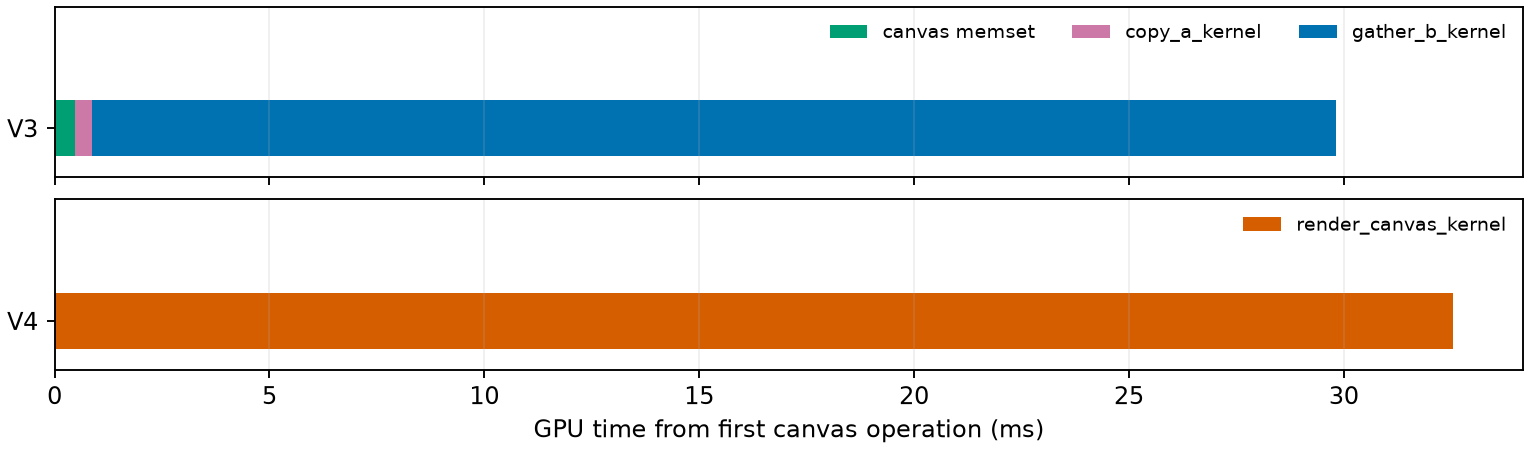
\includegraphics[width=.94\linewidth]{generated/nsys-v4.png}
\begin{itemize}
\item Tesla T4, site2/large, second pass of each trace.
\item V3 clear, copy A and gather B total 29.804 ms. V4 render takes 32.541 ms in this trace.
\item The five-run benchmark measures S6 at 28.712 ms for V3 and 28.190 ms for V4.
\end{itemize}
\end{frame}

\begin{frame}{Nsight Compute finds more DRAM traffic in sampled kernels}
\centering
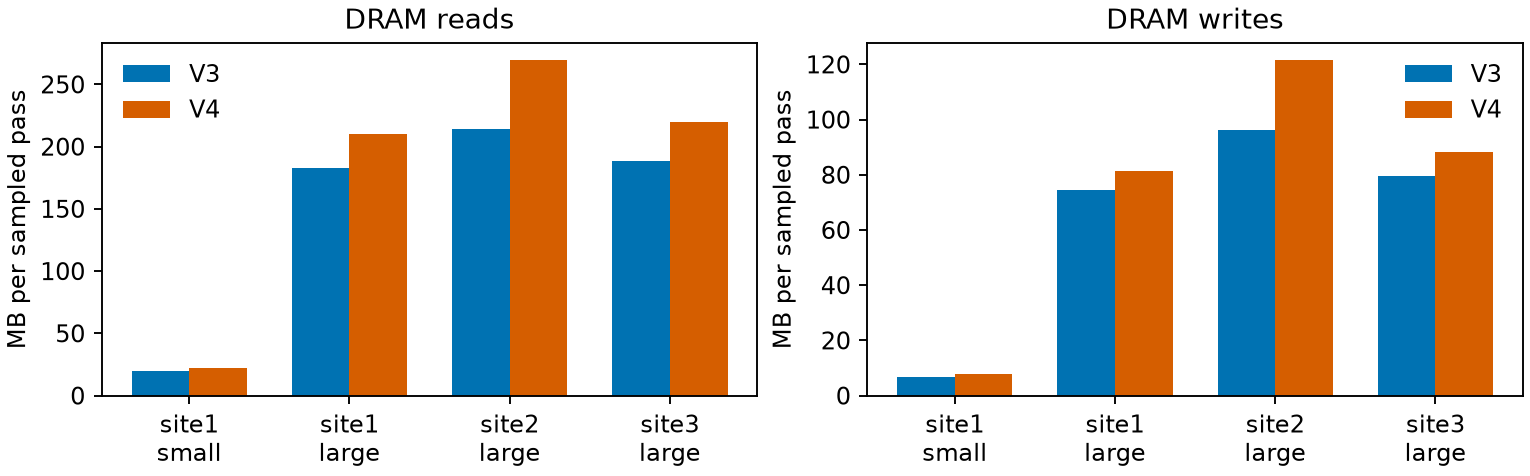
\includegraphics[width=.94\linewidth]{generated/ncu-v4.png}
\begin{itemize}
\item At site2/large, reads plus writes rise from 310.78 to 391.69 MB (+26.0\%).
\item The V3 bars sum one sample each of copy A and gather B. The V4 bars use one renderer sample. V3 canvas memset is outside the counter scope.
\end{itemize}
\end{frame}

\begin{frame}{What determines whether V4 is useful?}
\begin{itemize}
\item P9: V4 is faster in 8/9 standard cases; S6 geometric mean speedup is 1.0357$\times$.
\item Primary case paired blocks: median 1.0270$\times$, range 0.9774--1.0409$\times$; 4/5 blocks favor V4.
\item The primary case does not reach the previously proposed 5\% improvement threshold.
\item Keep challenge failures explicit; an absent timing is not zero time.
\item Separate profiler observations from unprofiled timing evidence.
\end{itemize}
\end{frame}

\begin{frame}{V5: dual-stream concurrency investigation}
\begin{block}{Two independent image branches}
Stream A and Stream B overlap H2D, S1, S2, and S3 concurrently; join before S4.
\end{block}
\begin{itemize}
\item Pre-S4 duration at site2/large decreases from $\sim$15.29 ms to $\sim$12.68 ms (1.207$\times$).
\item End-to-end speedup is modest (1.027$\times$ geometric mean) because downstream S5 and S6 dominate total time and SM resources are shared.
\item Confirms correctness and memory safety (0 memcheck errors, bit-for-bit parity with sequential mode).
\item Conclusion: V4 remains the production version; V5 serves as a concurrent stream case study.
\end{itemize}
\end{frame}

\begin{frame}{Lessons and limits}
\begin{itemize}
\item Faster S5 exposes S6; stage speedup is bounded by its pipeline share.
\item Fusion removes canvas passes. The sampled kernels show higher DRAM traffic.
\item Occupancy and throughput explain behavior; they are not the performance objective.
\item Preserve hashes, commands, raw runs, failures and original reports.
\item P9: total speedup is only 1.0086$\times$ (geometric mean); the benefit is modest.
\end{itemize}
\end{frame}
 from the shared Beamer document.
\begin{frame}{How the experiment is controlled}
\begin{itemize}
\item One Tesla T4 session; one pinned source and binary for V0--V4.
\item Official dataset: 3 standard sites, 3 resolutions, plus challenge cases.
\item One warm-up and 5 measured runs per successful configuration.
\item Report stages, H2D, D2H, kernel total, and end-to-end separately.
\item Compare speedups only within the same measurement session.
\end{itemize}
\end{frame}

\begin{frame}{APOD: follow the measured bottleneck}
\begin{description}
\item[Assess] Identify the dominant stage using timing and Nsight.
\item[Parallelize] V1 moves the six-stage pipeline to CUDA.
\item[Optimize] V2/V3 target S5; V4 targets canvas construction in S6.
\item[Deploy] Preserve correctness, check memory safety, retain evidence.
\end{description}
\medskip
An improved stage can expose a different pipeline bottleneck.
\end{frame}

\begin{frame}{Why investigate S6 after V3?}
\centering
\begin{tabular}{lrr}
\toprule
P8, site2/large & V2 & V3 \\
\midrule
S5 (ms) & 30.538 & 12.200 \\
S6 (ms) & 29.580 & 28.468 \\
Pipeline total (ms) & 81.826 & 62.353 \\
\bottomrule
\end{tabular}
\medskip
\begin{itemize}
\item S6 accounts for 45.7\% of the V3 total in this historical run.
\item Even a 2$\times$ S6 speedup would allow only about 1.30$\times$ total speedup if everything else stayed constant.
\end{itemize}
\tiny Source: P8 report, 16 Nov 2026, same-session V2/V3; source checkout b3c79d7. Historical context only; P9 remeasures all versions.
\end{frame}

\begin{frame}{V4: single-pass canvas fusion}
\begin{block}{V3 renderer}
Clear canvas $\rightarrow$ copy A $\rightarrow$ gather and blend B.
\end{block}
\begin{block}{V4 renderer}
One thread per output pixel: test A/B validity, sample source pixels, blend, write RGB once.
\end{block}
\begin{itemize}
\item Keep canvas geometry, inverse projection, interpolation and rounding rules.
\item Reuse S1--S4 from V1 and S5 from V3.
\item Fewer passes suggest less traffic; hardware counters must verify actual DRAM traffic.
\end{itemize}
\end{frame}

\begin{frame}{Correctness before performance}
\begin{itemize}
\item P9-T02: six synthetic pairs and twelve real configurations on Tesla T4.
\item Accepted V4 source: \texttt{ab8df98d}; benchmark checks source equivalence.
\item Ten successful real cases: matching geometry and Max RGB = 0.
\item Challenge medium/large preserve the expected S6 NumericalFailure status.
\item Suite and production CLI memcheck: zero errors, zero bytes leaked.
\end{itemize}
\medskip
\tiny Source: docs/report/p9-v4-verification.md. Acceptance timing is excluded from benchmark tables.
\end{frame}

\begin{frame}{V4 benchmark: same-session comparison}
% Generated from same-session P9 CSV; source ba97ed7, 2026-11-19.
\scriptsize
\centering
\begin{tabular}{llrrrr}
\toprule
Site & Size & V3 ms & V4 ms & Total speedup & S6 speedup \\
\midrule
site1 & small & 32.620 & 32.716 & 0.9971$\times$ & 1.0359$\times$ \\
site1 & medium & 31.027 & 30.785 & 1.0078$\times$ & 1.0633$\times$ \\
site1 & large & 108.107 & 107.157 & 1.0089$\times$ & 1.0061$\times$ \\
site2 & small & 21.415 & 21.142 & 1.0129$\times$ & 1.0368$\times$ \\
site2 & medium & 27.932 & 27.581 & 1.0127$\times$ & 1.0495$\times$ \\
site2 & large & 62.874 & 62.197 & 1.0109$\times$ & 1.0185$\times$ \\
site3 & small & 44.846 & 44.576 & 1.0061$\times$ & 1.0193$\times$ \\
site3 & medium & 56.167 & 55.723 & 1.0080$\times$ & 1.0403$\times$ \\
site3 & large & 101.713 & 100.393 & 1.0131$\times$ & 1.0525$\times$ \\
\bottomrule
\end{tabular}
\par\medskip Geometric mean total: 1.0086$\times$; S6: 1.0357$\times$.
\par One T4 session, one warm-up + 5 runs; nine standard cases.
\par\tiny Source: P9-T05, 19 Nov 2026, ba97ed7. Challenge failures excluded.

\end{frame}

\begin{frame}{Nsight Systems shows three canvas operations become one}
\centering
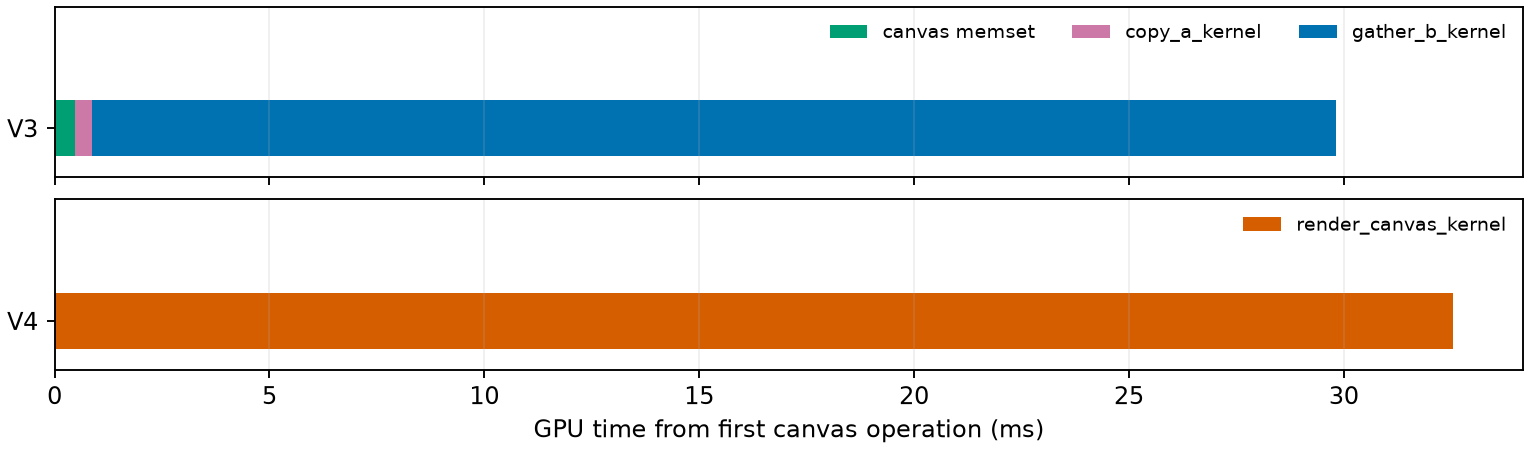
\includegraphics[width=.94\linewidth]{generated/nsys-v4.png}
\begin{itemize}
\item Tesla T4, site2/large, second pass of each trace.
\item V3 clear, copy A and gather B total 29.804 ms. V4 render takes 32.541 ms in this trace.
\item The five-run benchmark measures S6 at 28.712 ms for V3 and 28.190 ms for V4.
\end{itemize}
\end{frame}

\begin{frame}{Nsight Compute finds more DRAM traffic in sampled kernels}
\centering
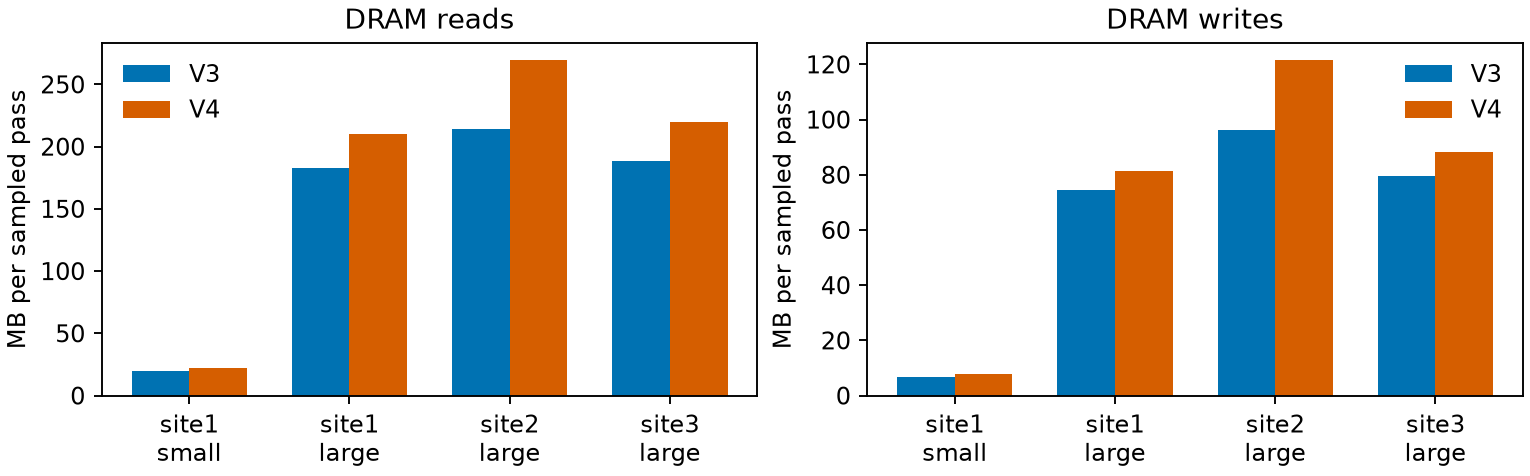
\includegraphics[width=.94\linewidth]{generated/ncu-v4.png}
\begin{itemize}
\item At site2/large, reads plus writes rise from 310.78 to 391.69 MB (+26.0\%).
\item The V3 bars sum one sample each of copy A and gather B. The V4 bars use one renderer sample. V3 canvas memset is outside the counter scope.
\end{itemize}
\end{frame}

\begin{frame}{What determines whether V4 is useful?}
\begin{itemize}
\item P9: V4 is faster in 8/9 standard cases; S6 geometric mean speedup is 1.0357$\times$.
\item Primary case paired blocks: median 1.0270$\times$, range 0.9774--1.0409$\times$; 4/5 blocks favor V4.
\item The primary case does not reach the previously proposed 5\% improvement threshold.
\item Keep challenge failures explicit; an absent timing is not zero time.
\item Separate profiler observations from unprofiled timing evidence.
\end{itemize}
\end{frame}

\begin{frame}{V5: dual-stream concurrency investigation}
\begin{block}{Two independent image branches}
Stream A and Stream B overlap H2D, S1, S2, and S3 concurrently; join before S4.
\end{block}
\begin{itemize}
\item Pre-S4 duration at site2/large decreases from $\sim$15.29 ms to $\sim$12.68 ms (1.207$\times$).
\item End-to-end speedup is modest (1.027$\times$ geometric mean) because downstream S5 and S6 dominate total time and SM resources are shared.
\item Confirms correctness and memory safety (0 memcheck errors, bit-for-bit parity with sequential mode).
\item Conclusion: V4 remains the production version; V5 serves as a concurrent stream case study.
\end{itemize}
\end{frame}

\begin{frame}{Lessons and limits}
\begin{itemize}
\item Faster S5 exposes S6; stage speedup is bounded by its pipeline share.
\item Fusion removes canvas passes. The sampled kernels show higher DRAM traffic.
\item Occupancy and throughput explain behavior; they are not the performance objective.
\item Preserve hashes, commands, raw runs, failures and original reports.
\item P9: total speedup is only 1.0086$\times$ (geometric mean); the benefit is modest.
\end{itemize}
\end{frame}
